	%\section{Experimentos}
	Neste capítulo são detalhados os experimentos que foram realizados sobre o sistema. Explanando como e onde os experimentos foram realizados, apresentando e detalhando os dados colhidos para enfim, analisa-los para no final do capítulo apresentar a conclusão.
	\\
	
	O objetivo dos experimentos é avaliar o desempenho do sistema sobre um ambiente de alta demanda, tanto com um único cliente quanto com múltiplas solicitações concorrentes. Para alcançar o primeiro caso, foram realizados \textbf{testes de latência} e para o último, \textbf{testes de \textit{throughput}}. Ambos os testes foram focados em apenas duas operações, leitura e escrita, sendo cada uma repetida para arquivos de quatro tamanhos distintos, 1KB, 100KB, 1MB e 10MB. Nas próximas seções estes experimentos serão descritos em maiores detalhes, porém, antes será apresentada uma breve descrição do ambiente de teste.
	\\
	
	\section{Ambiente de Teste}
	Os testes foram todos executados utilizando-se as facilidades da plataforma \textbf{Emulab-Net}, mais informações sobre a plataforma podem ser encontradas na página oficinal no endereço \href{https://www.emulab.net/}{https://www.emulab.net/}. Para este trabalho, basta saber que o Emulab-Net é uma ferramenta complexa para testes de rede com mais de 900 computadores (denominados como \textit{nodes}) separados em diferentes categorias que possibilitam o desenvolvimento de experimentos sofisticados nas áreas de rede de computadores e computação distribuída.
	\\
		
	\capstartfalse
	\begin{table} [htb]
		\caption{Especificações Técnicas das Máquinas}
		\centering
		\begin{tabular}{|l|l|} \hline
			\textbf{Descrição} 	& \textbf{Valor} \\ \hline
			
			Tipo				& d430\\ \hline
			Classe				& PC\\ \hline
			Sistema Operacional & Ubuntu (64bits)\\ \hline
			Disco Rígido		& 200GB \\ \hline
			Memória RAM			& 4GB \\ \hline
			Nº de \textit{Cores}& 8 \\ \hline
			Velocidade do CPU	& 2.4GHz  \\ \hline
						
		\end{tabular}
		\label{tab:exp_vm}
	\end{table}
	\capstarttrue
	
	Antes de se iniciar um experimento é necessário informar quantas e quais tipos de máquinas serão utilizados, além de modelar a topologia que deve ser utilizada entre os dispositivos na rede. 
	\\
	
	Para a realização dos experimentos foram solicitadas oito máquinas, onde três seriam utilizadas para execução do serviço de metadados, quatro para o serviço de armazenamento e a última para executar o lado do cliente. As especificações técnicas de cada uma das oito máquinas encontram-se registradas na Tabela~\ref{tab:exp_vm}. Enquanto que a Figura~\ref{fig:emulab} representa a topologia utilizada nos experimentos descritos nesse capítulo.
	\\
	
	\begin{figure}[htb]
		\begin{center}
			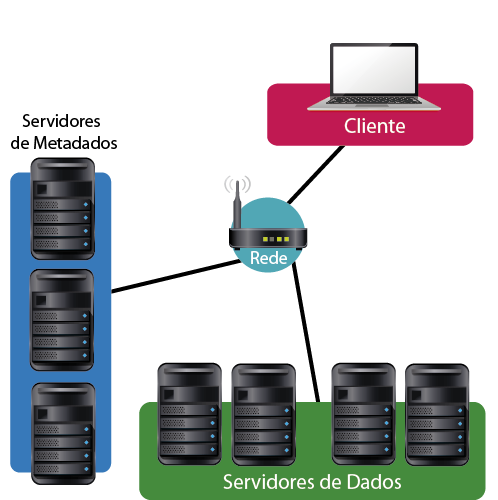
\includegraphics[clip,scale=0.5]{images/emulab.png}
			\caption{Topologia da rede nos experimentos.}
			\label{fig:emulab}
		\end{center}
	\end{figure} 
	

	\subsubsection{Teste de latência}
	O objetivo do teste de latência é mensurar o tempo total que o sistema leva para executar uma operação. Nesse experimento foram testadas apenas as operações de leitura e escrita de arquivos. Cada operação foi repetida 1000 vezes de forma consecutiva utilizando-se um arquivo fixo, sendo que esse procedimento foi executado com arquivos de tamanho de 1KB, 100KB, 1MB e 10MB. Todo esse procedimento foi repetido uma única vez para cada nível de RAID suportado pelo nosso sistema, ou seja, RAID 0, RAID 1 e RAID 5. Ao fim de cada execução desse procedimento os dados eram coletados e armazenados.
	\\
	
	\subsubsection{Teste de \textit{throughput}}	
	O objetivo do teste de \textit{throughput} é mensurar quantas operações o sistema consegue executar por segundo. Para tal, ele é realizado de forma extremamente simular ao teste de latência, a única diferença é o fato de não ser apenas um único cliente solicitando as operações, mas sim vários clientes concorrentes. Como na modelagem do experimento existe apenas uma máquina para o cliente, foram utilizadas várias \textit{threads} onde cada uma funciona como se fosse um cliente distinto. Ao fim de cada execução do procedimento os dados eram coletados e armazenados.
	\\
	
	O processo supracitado foi inicialmente realizado com 10 \textit{threads} e os dados coletados, em seguida repetiu-se o mesmo processo com 20 \textit{threads} e os dados coletados comparados com o caso anterior de 10 \textit{threads}. Essa operação foi repetida até chegar ao ponto máximo de \textit{threads} concorrentes em que o sistema respondia aumentando a vazão. O ponto máximo encontrado foi de 50 \textit{threads} concorrentes.
	\\